\documentclass[tikz,border=6pt]{standalone}
\usepackage[T1]{fontenc}
\usepackage{lmodern}
\usepackage{amsmath}
\usepackage{pgfplots}
\pgfplotsset{compat=1.18}
\usetikzlibrary{arrows.meta,positioning,fit,backgrounds,shapes.geometric,calc}
\definecolor{navy}{HTML}{16324F}
\definecolor{tealC}{HTML}{007F82}
\definecolor{amberC}{HTML}{D97706}
\definecolor{coralC}{HTML}{C2410C}
\definecolor{redC}{HTML}{DC2626}
\definecolor{mintC}{HTML}{059669}
\definecolor{slateC}{HTML}{64748B}
\definecolor{paleBg}{HTML}{F4F7FA}
\definecolor{softTeal}{HTML}{E6F4F4}
\definecolor{softNavy}{HTML}{EAF0F6}
\definecolor{softAmber}{HTML}{FEF3C7}
\begin{document}

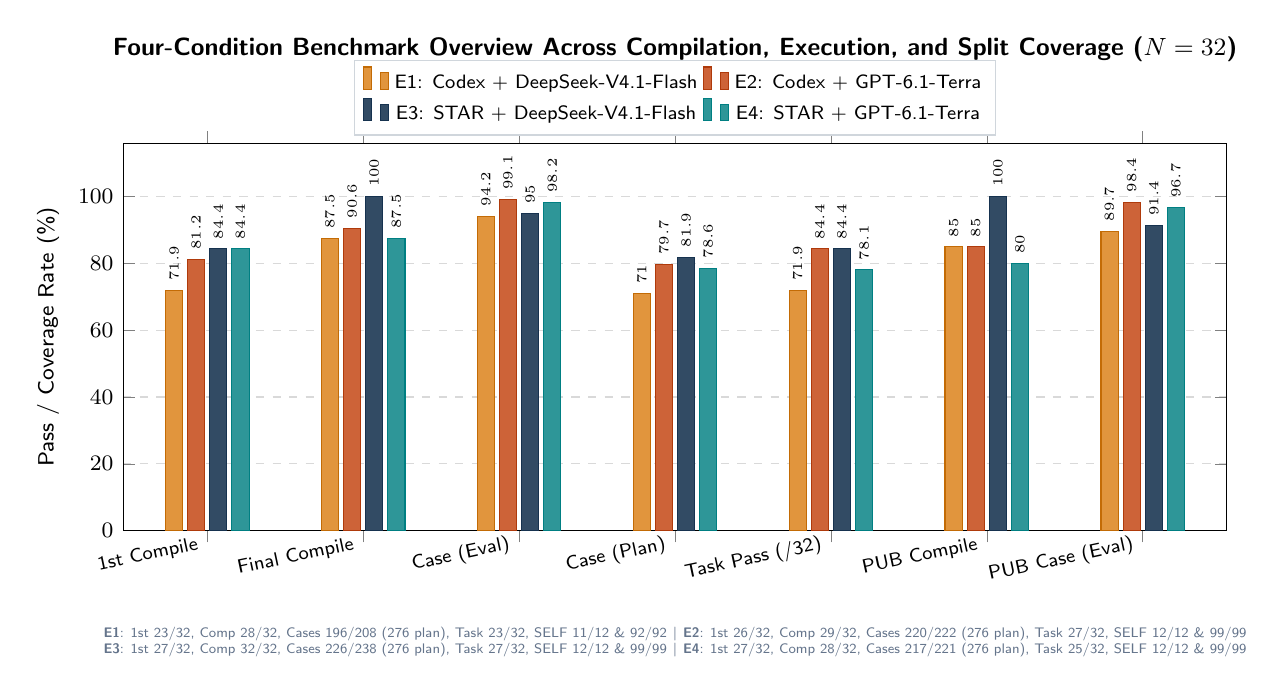
\begin{tikzpicture}
\begin{axis}[
    ybar=1.8pt,
    bar width=6.2pt,
    width=15.6cm,
    height=6.5cm,
    ymin=0, ymax=116,
    ylabel={\footnotesize Pass / Coverage Rate (\%)},
    xtick={0,1,2,3,4,5,6},
    xticklabels={{1st Compile},{Final Compile},{Case (Eval)},{Case (Plan)},{Task Pass (/32)},{PUB Compile},{PUB Case (Eval)}},
    x tick label style={font=\scriptsize\sffamily, rotate=12, anchor=east},
    ytick={0,20,40,60,80,100},
    tick label style={font=\footnotesize\sffamily},
    label style={font=\footnotesize\sffamily},
    title={\small\sffamily\bfseries Four-Condition Benchmark Overview Across Compilation, Execution, and Split Coverage ($N=32$)},
    title style={yshift=7mm},
    legend style={at={(0.5,1.02)}, anchor=south, legend columns=2, font=\scriptsize\sffamily, draw=navy!20, fill=white},
    nodes near coords,
    every node near coord/.append style={font=\tiny\sffamily, rotate=90, anchor=west},
    ymajorgrids=true,
    grid style={dashed, gray!30},
    enlarge x limits=0.09,
]
\addplot[fill=amberC!78, draw=amberC!90!black] coordinates {(0,71.9) (1,87.5) (2,94.2) (3,71.0) (4,71.9) (5,85.0) (6,89.7)};
\addplot[fill=coralC!82, draw=coralC!90!black] coordinates {(0,81.2) (1,90.6) (2,99.1) (3,79.7) (4,84.4) (5,85.0) (6,98.4)};
\addplot[fill=navy!88, draw=navy] coordinates {(0,84.4) (1,100.0) (2,95.0) (3,81.9) (4,84.4) (5,100.0) (6,91.4)};
\addplot[fill=tealC!82, draw=tealC] coordinates {(0,84.4) (1,87.5) (2,98.2) (3,78.6) (4,78.1) (5,80.0) (6,96.7)};
\legend{E1: Codex + DeepSeek-V4.1-Flash, E2: Codex + GPT-6.1-Terra, E3: STAR + DeepSeek-V4.1-Flash, E4: STAR + GPT-6.1-Terra}
\end{axis}
\node[font=\tiny\sffamily, color=slateC, anchor=north, align=center] at (current axis.south) [yshift=-11mm]
  {\textbf{E1}: 1st 23/32, Comp 28/32, Cases 196/208 (276 plan), Task 23/32, SELF 11/12 \& 92/92 $\mid$ \textbf{E2}: 1st 26/32, Comp 29/32, Cases 220/222 (276 plan), Task 27/32, SELF 12/12 \& 99/99\\\textbf{E3}: 1st 27/32, Comp 32/32, Cases 226/238 (276 plan), Task 27/32, SELF 12/12 \& 99/99 $\mid$ \textbf{E4}: 1st 27/32, Comp 28/32, Cases 217/221 (276 plan), Task 25/32, SELF 12/12 \& 99/99};
\end{tikzpicture}
\end{document}
